%%%%%%%%%%%%%%%%%%%%%%%%%%%%%%%%%%%%%%%%%
% Beamer Presentation
% LaTeX Template
% Version 1.0 (10/11/12)
%
% This template has been downloaded from:
% http://www.LaTeXTemplates.com
%
% License:
% CC BY-NC-SA 3.0 (http://creativecommons.org/licenses/by-nc-sa/3.0/)
%
%%%%%%%%%%%%%%%%%%%%%%%%%%%%%%%%%%%%%%%%%

%----------------------------------------------------------------------------------------
%	PACKAGES AND THEMES
%----------------------------------------------------------------------------------------

\documentclass{beamer}
\mode<presentation> {
\usetheme{Madrid}
}
\usepackage{url}
\usepackage{lmodern}
\usepackage{graphicx}
\usepackage{booktabs}

% for mathematics
\usepackage{amsmath}
\usepackage{amsthm}

%----------------------------------------------------------------------------------------
%	TITLE PAGE
%----------------------------------------------------------------------------------------

\title[Financial mathematics with Python]{UROPS Project Presentation 8} % The short title appears at the bottom of every slide, the full title is only on the title page

\author{Wang Zexin} % Your name
\institute[NUS]
{
Chapter 18 Portfolio Valuation\\
of Python for Finance\\[3mm]
\medskip
\textit{Quantitative Finance\\
National University of Singapore\\}
}
\date{\today}

\begin{document}
%----------------------------------------------------------------------------------------
%	TITLE PAGE
%----------------------------------------------------------------------------------------
\begin{frame}
\titlepage
\end{frame}

%----------------------------------------------------------------------------------------
%	TABLE OF CONTENTS
%----------------------------------------------------------------------------------------

%------------------------------------------------
\begin{frame}
\frametitle{Today's Agenda}
\tableofcontents
\end{frame}

%------------------------------------------------
\begin{frame}
\frametitle{Changes due to different Python version}
We are using Python 3.6 while the version in the book is Python 2.7\\
So here is a list of items to change\\[2mm]
\begin{itemize}
	\item print x now becomes print(x)
	\item dict.iteritems() now becomes dict.items()
	\item xrange now becomes range
	\item lambda (k, v) : (v, k) is no longer available
	\item instead we can only use: lambda x : (x[1], x[0])
	\item x / 2 is float division, while x // 2 is integer division
\end{itemize}
\end{frame}

%------------------------------------------------
\section{Portfolio Valuation}

%------------------------------------------------
\begin{frame}
\frametitle{Derivatives Valuation}
\begin{itemize}
	\item Generic Valuation Class\\[3mm]
	\item Numerical Evaluation of Greeks\\[3mm]
	\item European Exercise\\[3mm]
	\item American Exercise\\[3mm]
	\item Wrapper class
\end{itemize}
\end{frame}

\subsection{General Modularization}

%------------------------------------------------
\begin{frame}
\frametitle{General Modularization}
The almost complete modularization of the analytics library:\\
(Based on Monte Carlo simulation being the only numerical method)
\begin{itemize}
	\item Discounting - $constant\_short\_rate$
	\item Relevant data - $market\_environment$
	\item Simulation objects
	\begin{itemize}
		\item geometric\_brownian\_motion
		\item jump\_diffusion
		\item square\_root\_diffusion
	\end{itemize}
	\item Valuation objects
	\begin{itemize}
		\item valuation\_mcs\_european
		\item valuation\_mcs\_american
	\end{itemize}
	\item Nonredundancy
	\item Correlations
	\item Positions
\end{itemize}
\end{frame}

%------------------------------------------------
\begin{frame}
\frametitle{Initialization}
The derivatives valuation class will include these attributes:\\
Quantity, Underlying, 
\begin{figure}[H]
	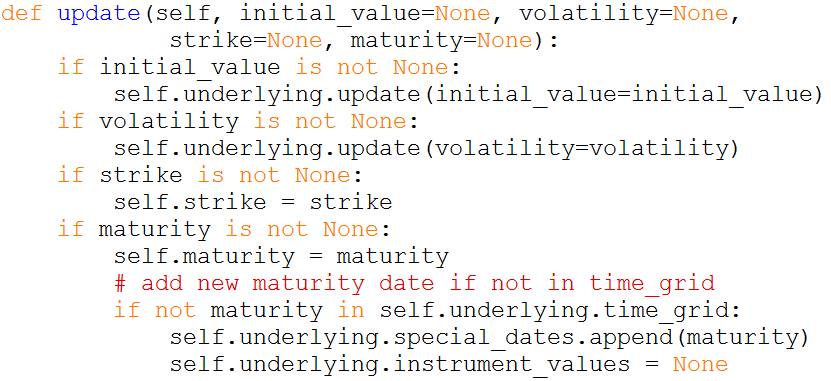
\includegraphics[scale=0.5]{update_valuation_class.png}
\end{figure}
\end{frame}

\subsection{Numerical Evaluation of Greeks}
%------------------------------------------------
\begin{frame}
\frametitle{Numerical Evaluation of Greeks}
Delta:
$$\Delta = \lim_{{^{\Delta}S} \to 0} \frac{V(S_{0}+{^{\Delta}S},\sigma_{0}) - V(S_{0}, \sigma_{0})}{^{\Delta}S} = \frac{\partial V}{\partial S}$$
Vega:
$$\nu = \lim_{{^{\Delta}\sigma} \to 0} \frac{V(S_{0},\sigma_{0}+{^{\Delta}\sigma}) - V(S_{0}, \sigma_{0})}{^{\Delta}\sigma} = \frac{\partial V}{\partial \sigma}$$
The sensitivity of the derivatives price to underlying price as well as to volatility can be numerically computed.
\end{frame}

%------------------------------------------------
\begin{frame}
\frametitle{Numerical Evaluation of $\Delta$}
This implementation calculates the change in derivatives value with respect to 2\% change in underlying asset price. (Can 2\% be too much?)
\begin{figure}[H]
	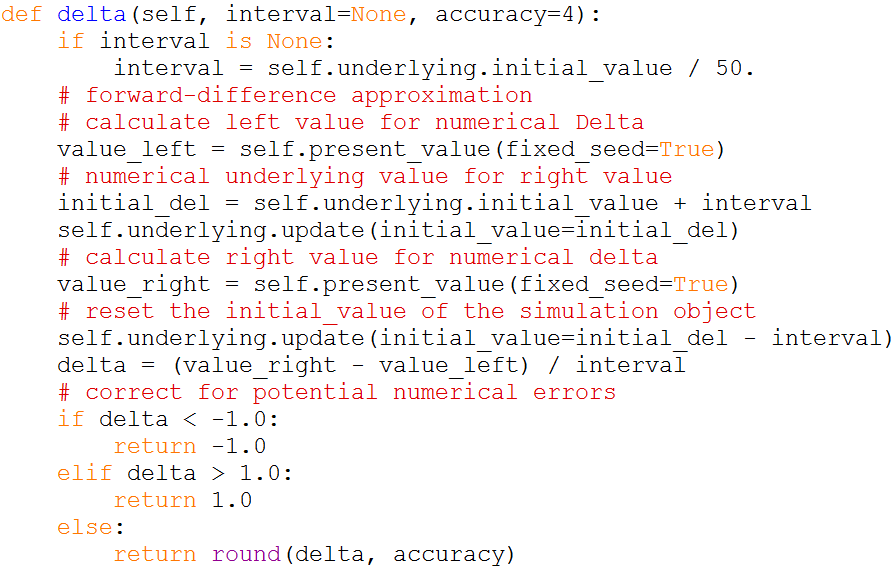
\includegraphics[scale=0.44]{delta_valuation_class.png}
\end{figure}
\end{frame}

%------------------------------------------------
\begin{frame}
\frametitle{Numerical Evaluation of $\nu$}
This implementation calculates the change in derivatives value with respect to 2\% change in volatility. (How can we correct for potential numerical errors?)
\begin{figure}[H]
	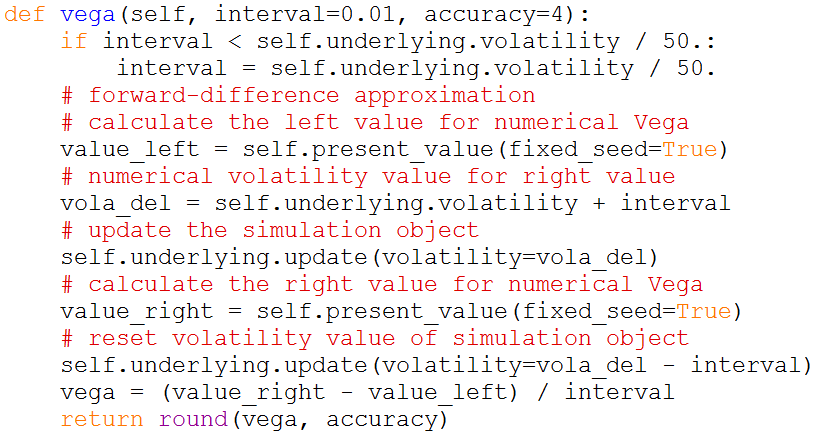
\includegraphics[scale=0.45]{vega_valuation_class.png}
\end{figure}
\end{frame}

\subsection{European Exercise}
%------------------------------------------------
\begin{frame}
\frametitle{European Exercise Generate Payoff}
If self.strike is not initiated, there will still be errors.\\
Also, computation using the $eval$ function can be slow.
\begin{figure}[H]
	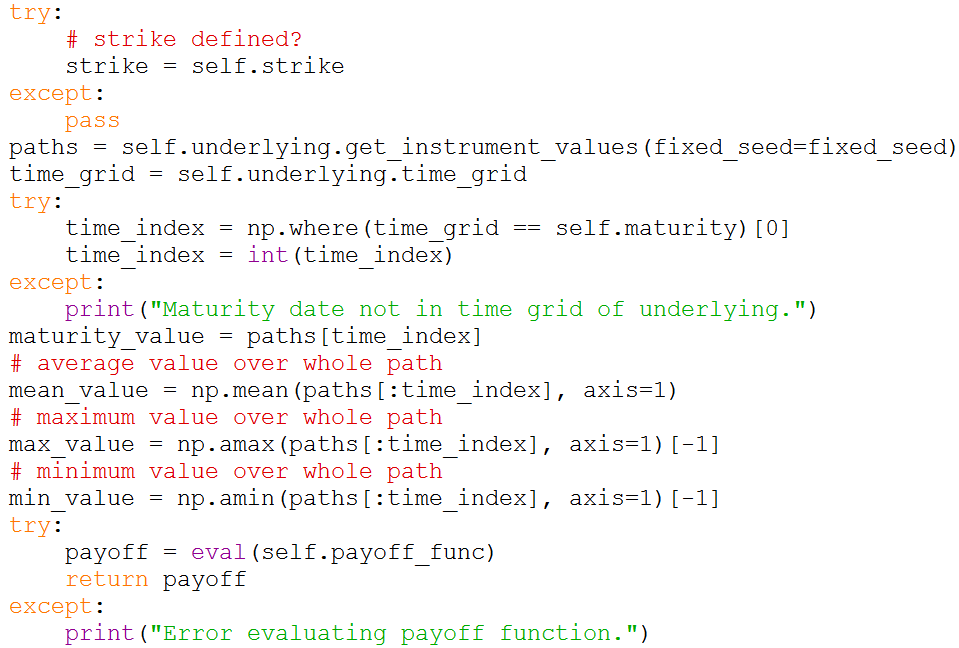
\includegraphics[scale=0.39]{european_generate_payoff.png}
\end{figure}
\end{frame}

%------------------------------------------------
\begin{frame}
\frametitle{European Exercise Valuation}
Calculate present value by discounting the expectation of payoff.
\begin{figure}[H]
	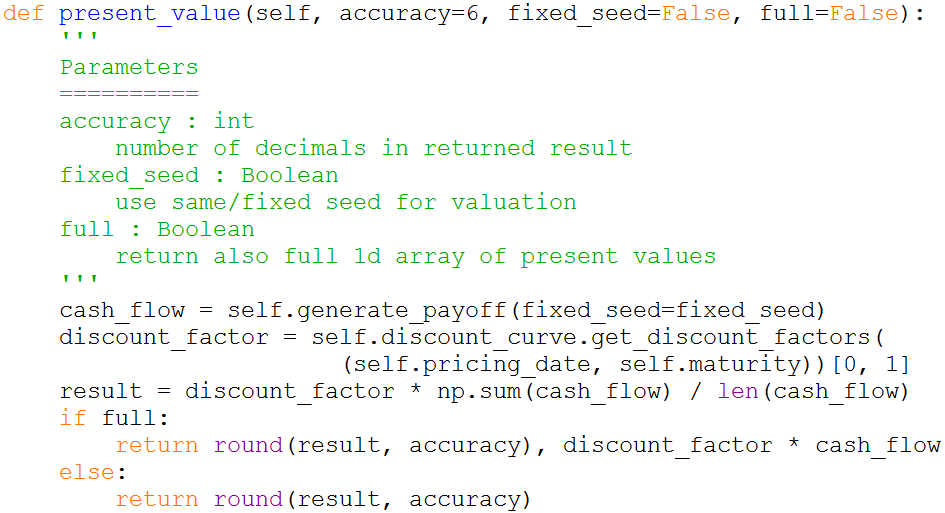
\includegraphics[scale=0.45]{european_present_value.png}
\end{figure}
\end{frame}

%------------------------------------------------
\begin{frame}
\frametitle{European Exercise User Case}
Assuming the attributes are correctly updated, for an European call option with $S_{0} = 36$, $\sigma = 0.2$ and $K = 40$, we may obtain the following:
\begin{figure}[H]
	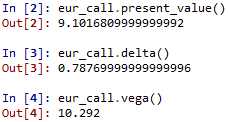
\includegraphics[scale=1.0]{european_exercise_user_case.png}
\end{figure}
\end{frame}

\subsection{American Exercise}
%------------------------------------------------
\begin{frame}
\frametitle{American Exercise Generate Payoff}
This function will pass out the time points of the optimal exercise price.
\begin{figure}[H]
	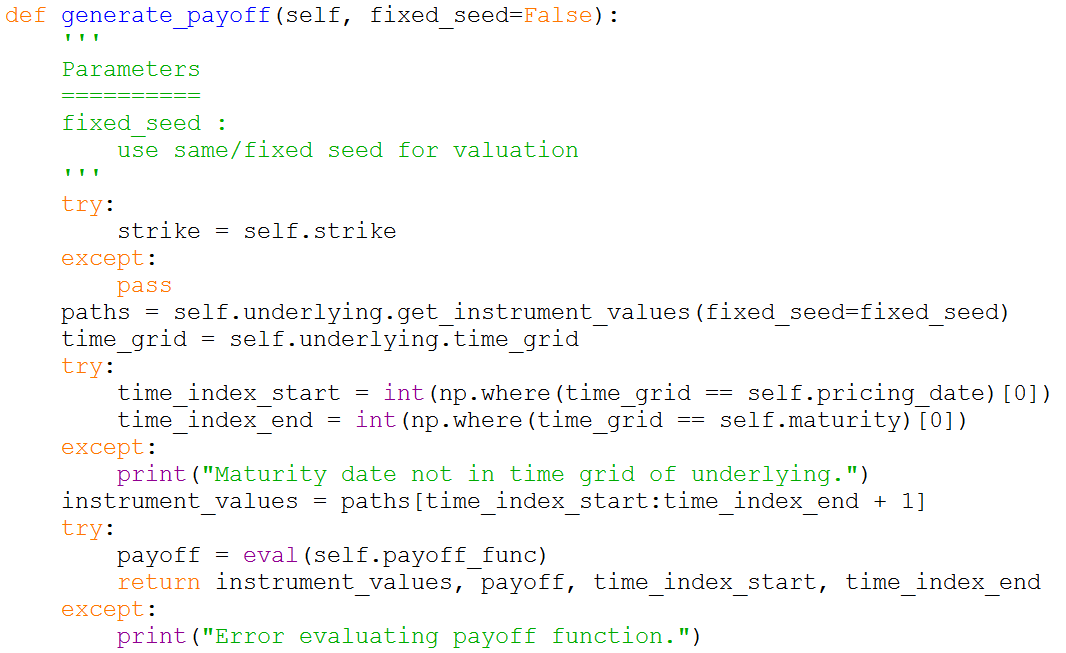
\includegraphics[scale=0.4]{american_generate_payoff.png}
\end{figure}
\end{frame}

%------------------------------------------------
\begin{frame}
\frametitle{American Exercise Valuation}
Fixed seed: same randomized values for separation simulations.\\
This function will derive different discount factors for different time points.
\begin{figure}[H]
	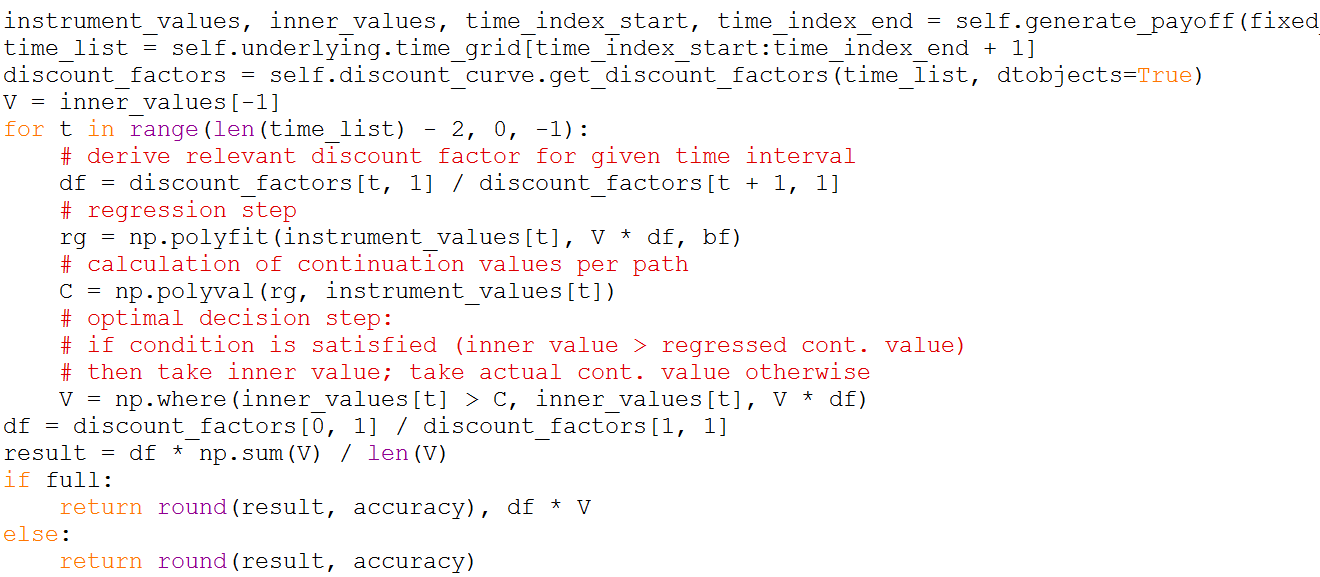
\includegraphics[scale=0.4]{american_present_value.png}
\end{figure}
\end{frame}

%------------------------------------------------
\begin{frame}
\frametitle{American Exercise User Case}
Assuming the attributes are correctly updated, for an American call option with $S_{0} = 36$, $\sigma = 0.2$ and $K = 40$, we may obtain the following:
\begin{figure}[H]
	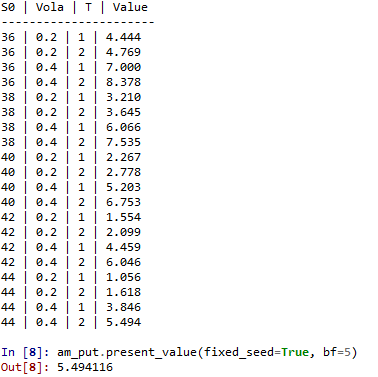
\includegraphics[scale=0.6]{american_exercise_user_case.png}
\end{figure}
\end{frame}

\subsection{Wrapper class}
%------------------------------------------------
\begin{frame}
\frametitle{Wrapper class - implementation}
\begin{figure}[H]
	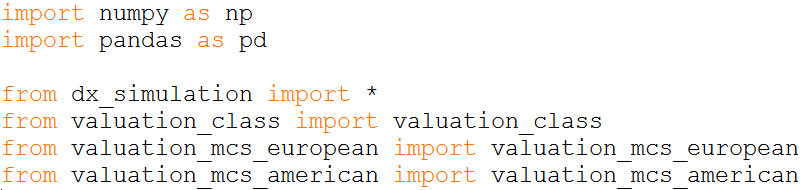
\includegraphics[scale=0.48]{wrapper_class.png}
\end{figure}
With this $dx\_valuation.py$, we are now able to import the valuation framework package as well the simulation classes in one line.
\end{frame}

%------------------------------------------------
\begin{frame}
\frametitle{Wrapper class - testing}
Now we need to enhance the $\_\_init\_\_.py$ which initially has the same content as $dx\_frame.py$ and $dx\_simulation.py$ in the same directory to include importing the simulation classes.
\begin{figure}[H]
	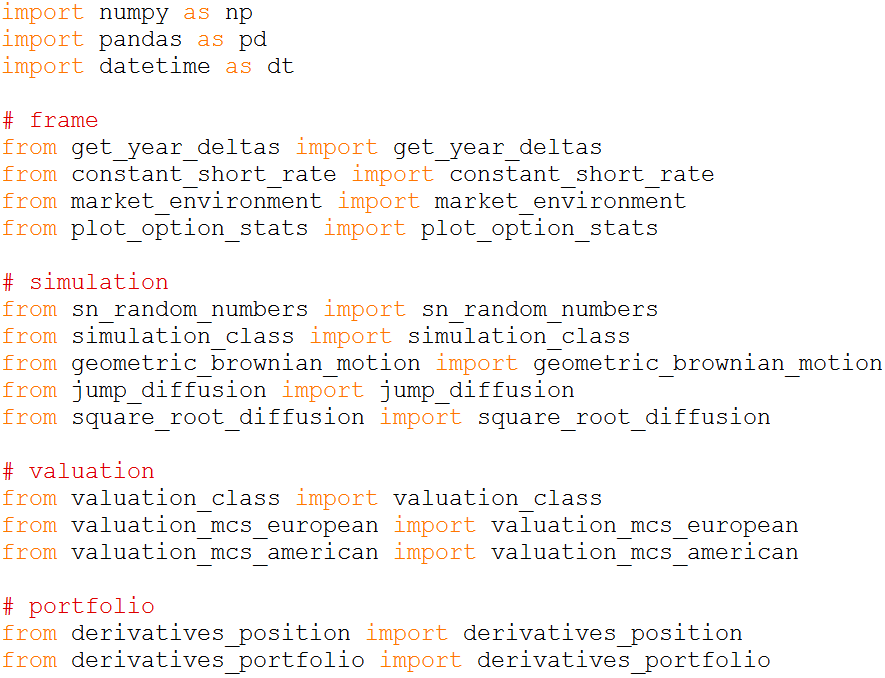
\includegraphics[scale=0.48]{overall_wrapper_class.png}
\end{figure}
\end{frame}

%-----------------------------------------------
\begin{frame}
\Huge{\centerline{Thank You}}
\begin{center}
\begin{normalsize}
\emph{E0007424@u.nus.edu}
\end{normalsize}
\end{center}
\end{frame}

%------------------------------------------------

\end{document} 